\section{Results}
In the following figures, the blue line represents the desired position caculated by the trajectory generator with the given path. To ensure the quadrotor stay relatively horizontal while flying. We limit the acceleration along x, y, z direction, so the performance of the quadrotor will be stable. 

Figure 1 is the 3D view of example 1. Figure 2, Figure 3, and Figure 4 are the results of 3 different views for example 1. The largest acceleration for this example is $0.3m^2/s$. 
\begin{figure}[H]
  \centering
  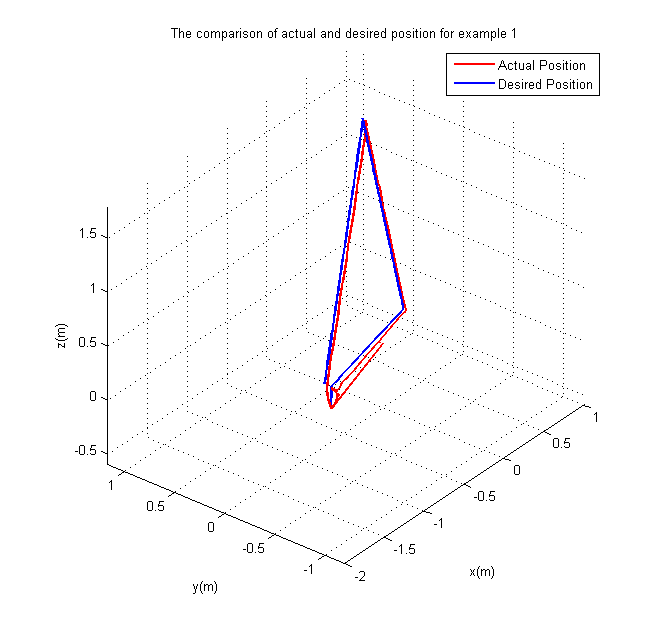
\includegraphics[width=3in]{Ex1_03_3D.png}
  \caption{3D view for example 1}
\end{figure}

\begin{figure}[H]
  \centering
  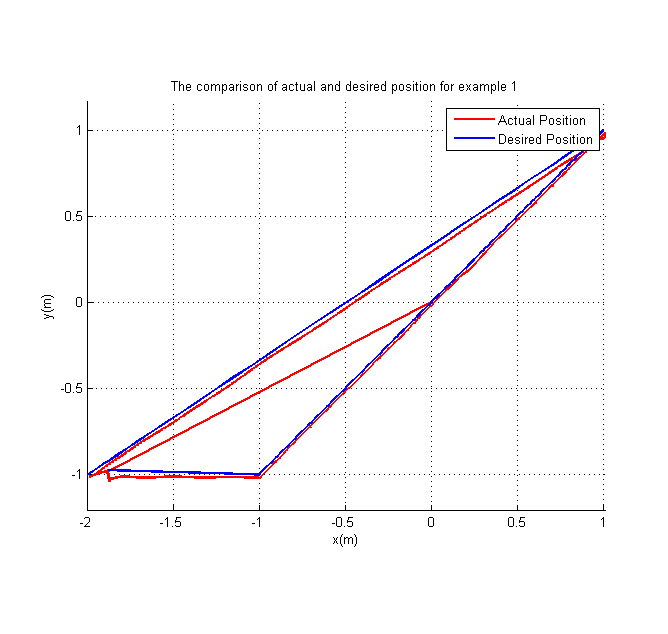
\includegraphics[width=3in]{Ex1_03_XY.PNG}
  \caption{Results of example1 in XY plane}
\end{figure}

\begin{figure}[H]
  \centering
  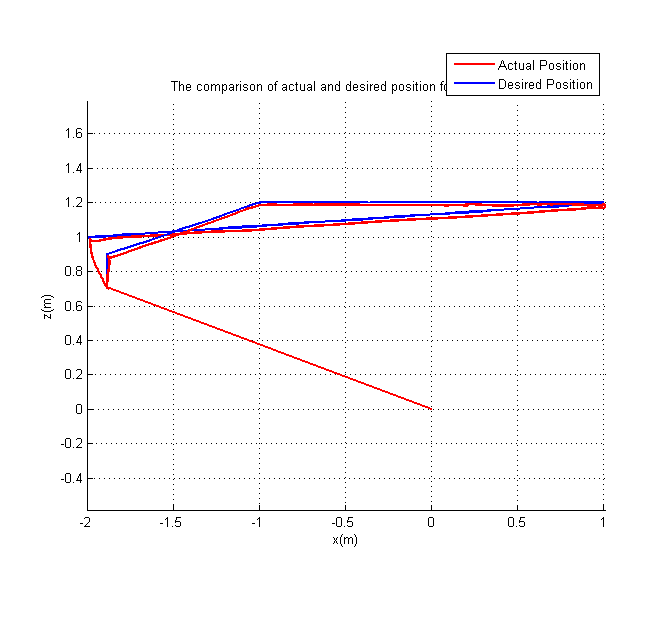
\includegraphics[width=3in]{Ex1_03_XZ.PNG}
  \caption{Results of example1 in XZ plane}
\end{figure}

\begin{figure}[H]
  \centering
  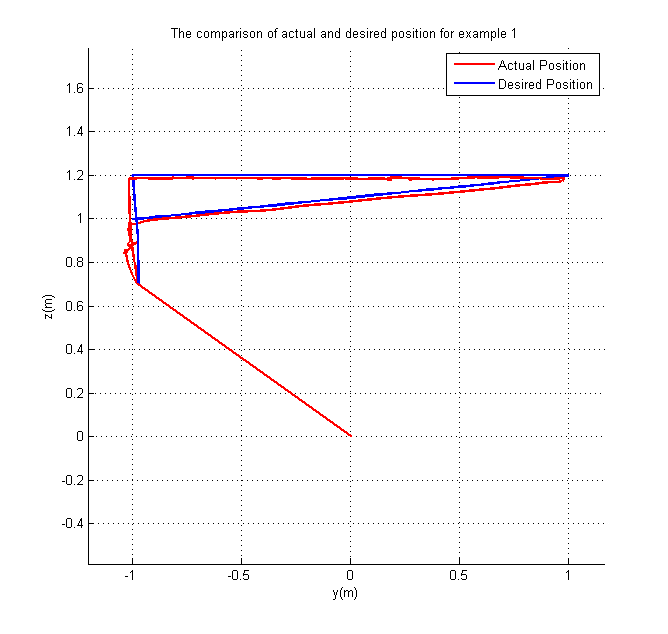
\includegraphics[width=3in]{Ex1_03_YZ.PNG}
  \caption{Results of example1 in YZ plane}
\end{figure}

Figure 5 to Figure 8 are the results from example 2 with a largest acceleration of $1m^2/s$ and Figure 9 to Figure 12 are also the results from example 2 but with a higher acceleration limitation of $3m^2/s$.
\begin{figure}[H]
  \centering
  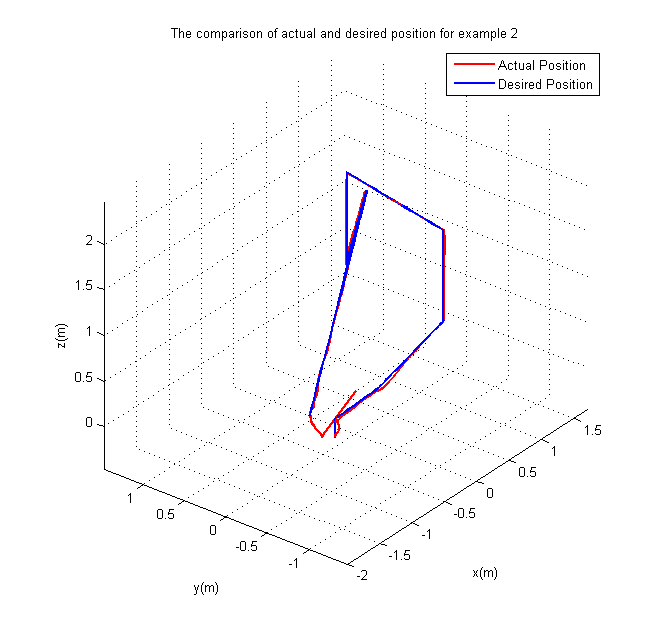
\includegraphics[width=3in]{Ex2_1_3D.png}
  \caption{3D view for example 2 with a lower acceleration}
\end{figure}

\begin{figure}[H]
  \centering
  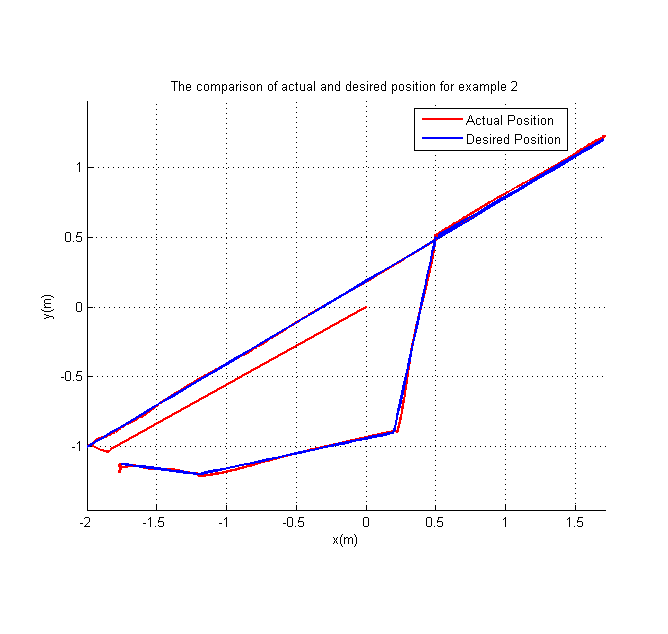
\includegraphics[width=3in]{Ex2_1_XY.PNG}
  \caption{Results of example2 in XY plane with a lower acceleration}
\end{figure}

\begin{figure}[H]
  \centering
  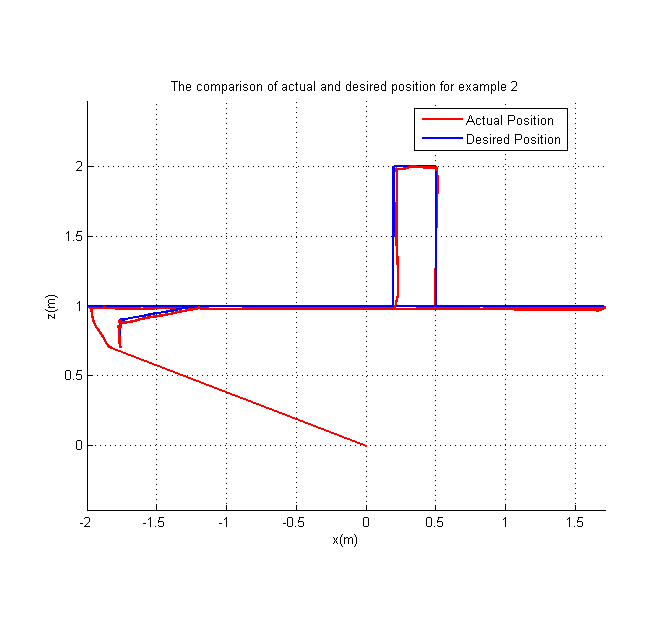
\includegraphics[width=3in]{Ex2_1_XZ.PNG}
  \caption{Results of example2 in XZ plane with a lower acceleration}
\end{figure}

\begin{figure}[H]
  \centering
  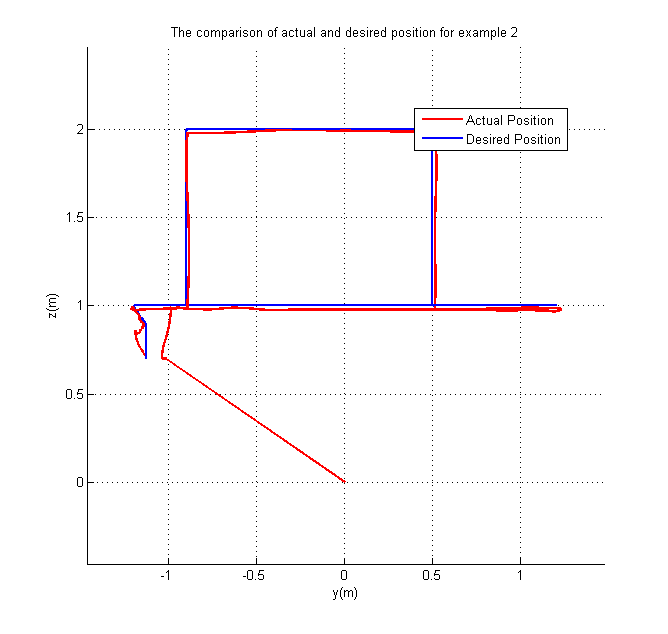
\includegraphics[width=3in]{Ex2_1_YZ.PNG}
  \caption{Results of example2 in YZ plane with a lower acceleration}
\end{figure}

\begin{figure}[H]
  \centering
  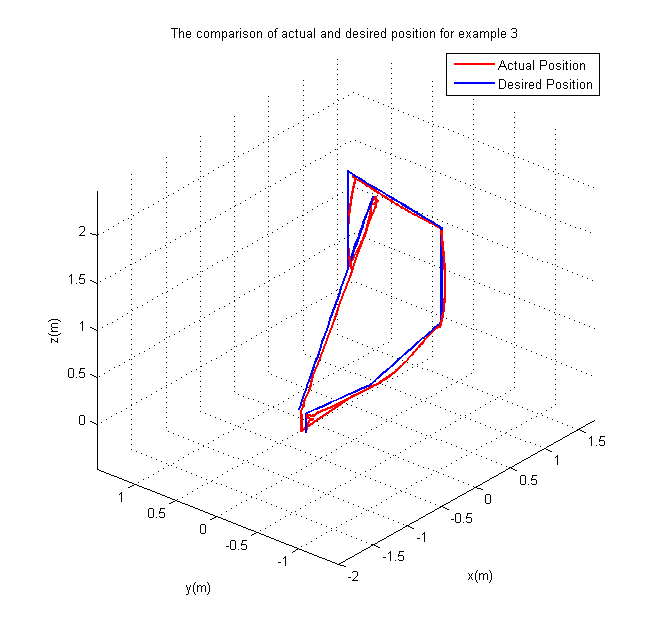
\includegraphics[width=3in]{Ex2_3_3D.png}
  \caption{3D view for example 2 with a higher acceleration}
\end{figure}

\begin{figure}[H]
  \centering
  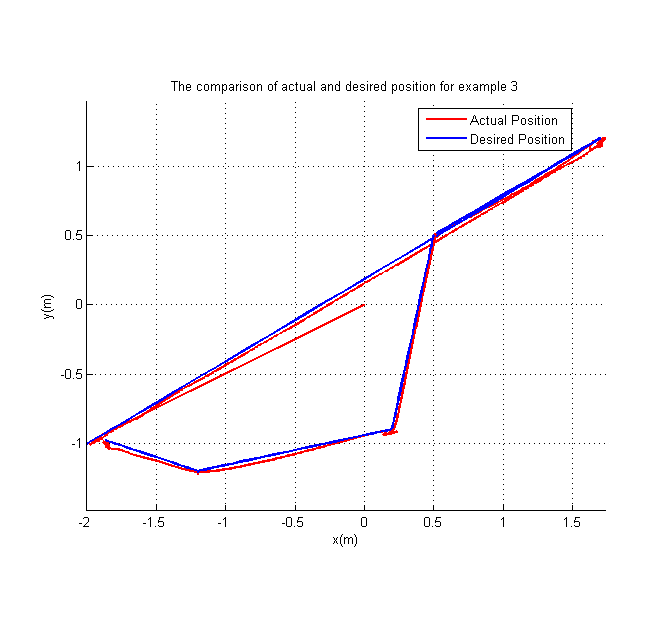
\includegraphics[width=3in]{Ex2_3_XY.PNG}
  \caption{Results of example2 in XY plane with a higher acceleration}
\end{figure}

\begin{figure}[H]
  \centering
  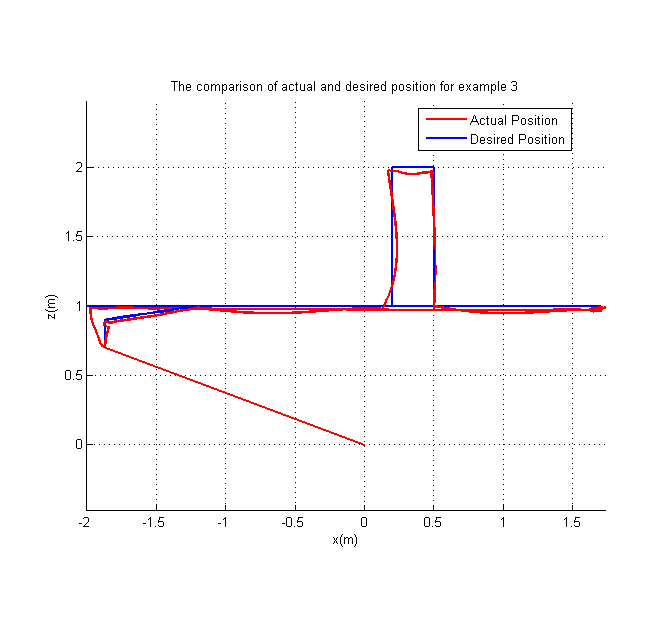
\includegraphics[width=3in]{Ex2_3_XZ.PNG}
  \caption{Results of example2 in XZ plane with a higher acceleration}
\end{figure}

\begin{figure}[H]
  \centering
  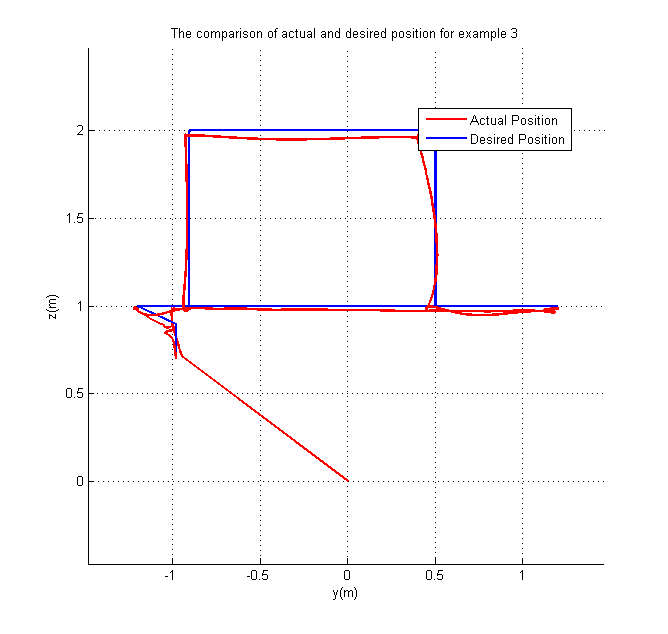
\includegraphics[width=3in]{Ex2_3_YZ.PNG}
  \caption{Results of example2 in YZ plane with a higher acceleration}
\end{figure}

The three views of example 3 are showed in Figure 14, Figure 15 and Figure 16. The 3D view of example 3 is showed in Figure 13.
\begin{figure}[H]
  \centering
  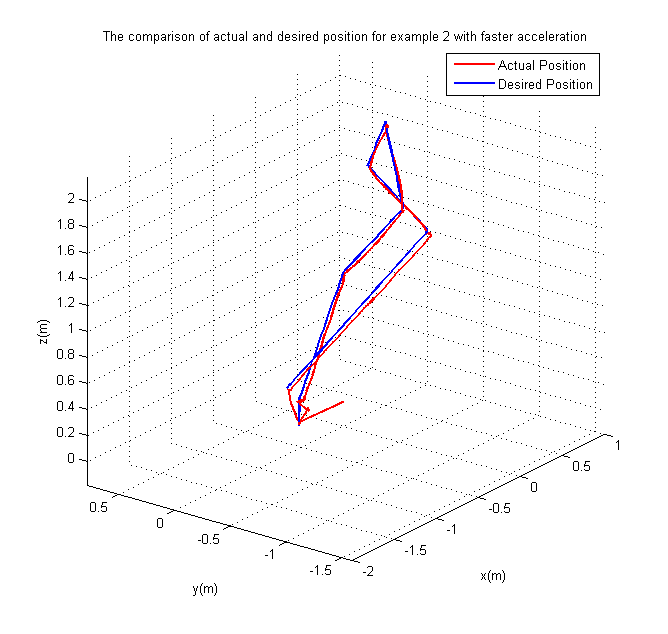
\includegraphics[width=3in]{Ex3_1_3D.png}
  \caption{3D view for example 3}
\end{figure}


\begin{figure}[H]
  \centering
  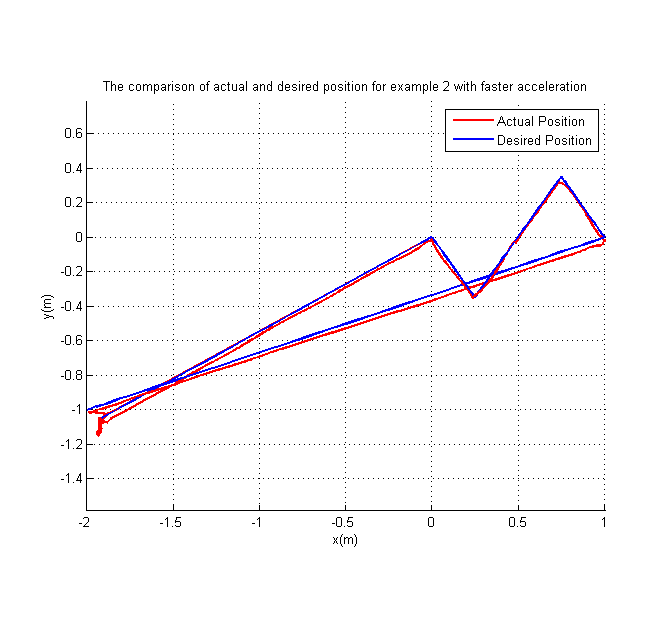
\includegraphics[width=3in]{Ex3_1_XY.PNG}
  \caption{Results of example1 in XY plane}
\end{figure}

\begin{figure}[H]
  \centering
  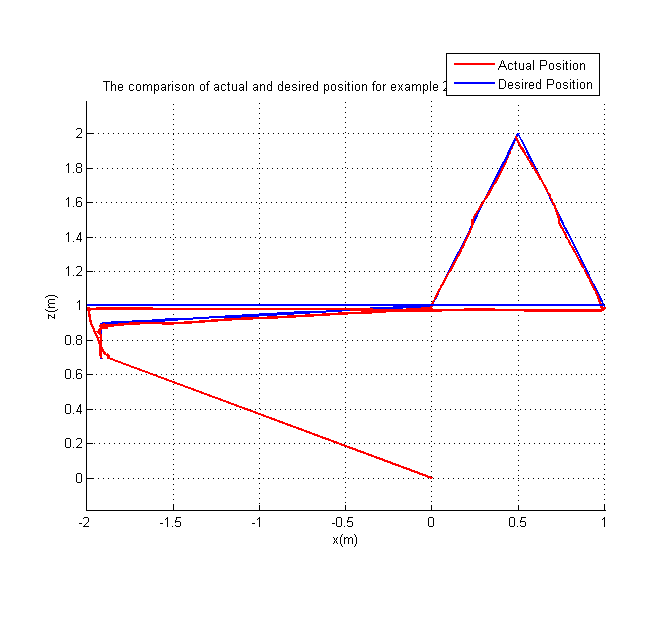
\includegraphics[width=3in]{Ex3_1_XZ.PNG}
  \caption{Results of example1 in XZ plane}
\end{figure}

\begin{figure}[H]
  \centering
  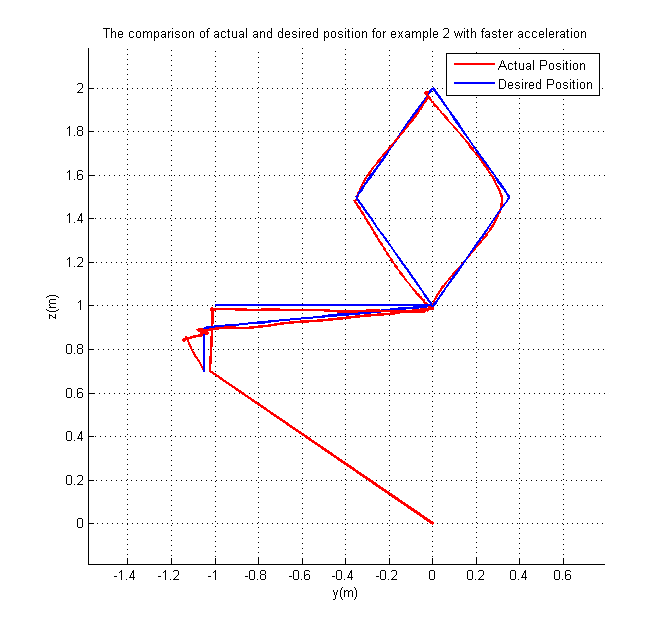
\includegraphics[width=3in]{Ex3_1_YZ.PNG}
  \caption{Results of example1 in YZ plane}
\end{figure}

The plots give us clear views for the desired trajectory and the real path recorded by Vicon. The quadrotor follows the blue path quite well. In example 2, we tried a higher speed by giving the controller a higher acceleration. Although the real path does not match the desired trajectory that good in the faster case, it still finish the flying quite stable. So, our controller is qualified for a flying at high speed.
\end{document}